\documentclass[12pt]{article}
% 
%\usepackage{tabularx}  
%\usepackage[dvips]{graphicx}
%\usepackage{longtable}
%\usepackage{hhline}
%\usepackage{alltt}
%\usepackage{ifthen}
\usepackage{epsfig}
%\usepackage{color}
%\usepackage{amsmath}
%\usepackage{tabularx}
%\usepackage{latexsym}
%
\def\1035{10$^{35}$~cm$^{-2}$s$^{-1}$}
\def\degg{$^{\circ}$ }
\def\qsq{$Q^2 $}
\def\co2{$CO_2 $}
\def\microns{$\mu m $ }
\def\gevcsq{$GeV/c^2 $}
\def\gev{$GeV $}
\def\gevc{$GeV/c $}
\usepackage{fancyhdr}
\topmargin -0.3in
\headheight 0.0in
\headsep 0.5in
\textheight 9.4in
\oddsidemargin -.0in
\evensidemargin -.0in
\textwidth 6.6in
\renewcommand{\baselinestretch}{1.4}
%

%\pagestyle{empty}       %suppresses page numbers
%
\begin{document}

\title{CLAS12 Drift Chambers}

\author{CLAS12 Drift Chamber Group\\ [0.5ex]
Jefferson Laboratory}

\maketitle

\vspace{2cm}
\begin{figure}[ht]
\begin{center}
\vspace{1cm}
\epsfig{file=umbrella.ps,width=11cm}
\end{center}
\end{figure}

\vfil
\eject

\tableofcontents

\vfil
\eject
\fancypagestyle{myheading}{%                % Redefining plain style
\fancyhf{} % clear all header and footer fields
\fancyhead[C]{\vspace{0.5cm}\line(1,0){500}\vspace{-0.5cm}}
\fancyhead[l]{\mbox{\bfseries CLAS12 Technical Design Report}}
\fancyhead[r]{\mbox{\bfseries Version 1.1  \date{\today}}}
\fancyfoot[C]{\mbox{\bfseries  \thepage }}
\fancyfoot[r]{\mbox{\bfseries Drift chambers}}
\fancyfoot[l]{\vspace{-1cm}\line(1,0){500}}
}
\renewcommand{\headrulewidth}{0pt}
\renewcommand{\footrulewidth}{0pt}
\pagestyle{myheading}


\section{CLAS12 Physics Requirements}

The {\tt CLAS} detector in Hall B is being upgraded to take advantage 
of the increase of the CEBAF beam energy from 6 to 12~GeV, thus the 
new name, {\tt CLAS12}.  There are several broad areas of physics 
enquiry that drive these changes: spectroscopic studies of excited 
baryons, investigations of the influence of nuclear matter on propagating 
quarks, studies of polarized and unpolarized quark distributions, and a 
comprehensive measurement of generalized parton distributions (GPDs).  
Many of the reactions of interest are electroproduction of exclusive and 
semi-inclusive final states.  The cross sections for these processes are 
small, necessitating high-luminosity experiments.  A variety of proposed 
experiments rely on luminosities of \1035 to achieve the desired statistical 
accuracy in runs of a few months duration.  The deep exclusive reactions in 
which an electron scattering at moderate to high values of $Q^2$ results in 
a meson-baryon final state, provide the most stringent requirements for 
the {\tt CLAS12} tracking system.  A final state of a few high-momentum, 
forward-going particles (the electron as well as one or more mesons), 
combined with a moderate-momentum baryon emitted at large angles, is the 
typical event type on which the specifications of the tracking system are 
based.  

In broad strokes, the tracking system must measure forward-going particles 
down to lab angles as small as 5$^{\circ}$ and as large as 
40$^{\circ}$ in order to cover as much of the hadronic center-of-mass 
region as possible.  A silicon strip tracking system will cover the 
40$^\circ$ - 135$^\circ$ angular range.  We require very good momentum and 
angular resolution for the scattered electron (on the order of 
$\Delta p/p = 1\%$ and $\Delta \theta$ = 1~mrad) in order to determine the 
virtual photon flux factor $\Gamma_v$, and hence the cross sections, to an 
accuracy of a few percent.  In addition, a momentum resolution of about 
20 to 50~MeV is necessary in order to positively identify a missing hadron 
in these exclusive reactions.  Finally, good vertex resolution will allow 
detection of secondary decay vertices and serve as a good marker for 
strangeness production.

A tracking system capable of achieving these standards was described
in the PCDR~\cite{pcdr} and quantitatively parameterized in a ``fast'' 
Monte Carlo (FASTMC) program~\cite{fastmc}.  A number of {\tt CLAS} 
collaborators used the existing model of the detector as described in 
{\tt FASTMC} in proposals presented to JLab PAC-30~\cite{pac30} in 
August 2006, the first PAC to consider 12-GeV proposals.



\section{Overview of the CLAS12 Detector}

In Fig.~\ref{clas12} we show a CAD model picture of the proposed 
{\tt CLAS12} detector highlighting each of the detector subsystems, 
including the three forward-angle drift chambers, called Regions 1, 2, 
and 3, as well as the central silicon vertex tracker.  
Table~\ref{tracker-specs} provides a listing of the {\tt CLAS12} tracking 
system design requirements.  {\tt CLAS12} is being designed to operate at 
a luminosity of \1035.  This higher luminosity goal (the present {\tt CLAS} 
detector operates at a maximum luminosity of 10$^{34}$~cm$^{-2}$s$^{-1}$) 
necessitates the use of a solenoidal magnet and conical absorber to shield 
the detector from M{\o}ller electrons.  To reduce interactions between this 
solenoidal field and the main {\tt CLAS} toroidal field, and to facilitate 
construction and installation of new detector elements, the torus has been 
re-designed.  It is more compact than the present torus while providing 
equivalent bending power for charged particles between 5$^{\circ}$ and 
40$^{\circ}$.

\vfil
\eject

%%%%%%%%%%%%%%%%%%%%%%%%%%%%%%%%%%%%%%%%%%%%%%%%%%%%%%%%%%%%%%%%%%%%%%%%%
\begin{figure}[htbp]
\vspace{11.0cm}
\special{psfile=clas12_system.eps hscale=70 vscale=70 hoffset=0 voffset=0}
\caption{\small{A three-dimensional view of the proposed {\tt CLAS12} 
detector highlighting the various subsystems.  The small inset on the left
shows the same area highlighted by the dashed box on the right but with
the solenoid removed to show the SVT system.}}
\label{clas12}
\end{figure}
%%%%%%%%%%%%%%%%%%%%%%%%%%%%%%%%%%%%%%%%%%%%%%%%%%%%%%%%%%%%%%%%%%%%%%%%%

%%%%%%%%%%%%%%%%%%%%%%%%%%%%%%%%%%%%%%%%%%%%%%%%%%%%%%%%%%%%%%%%%%%%%%%%%
\begin{table}[htbp]
\begin{center}
\begin{tabular} {||c|c||} \hline \hline
{\bf Category}      & {\bf Requirement} \\ \hline
Angular coverage    & 5$^{\circ}$ - 135$^{\circ}$ \\ \hline
Momentum resolution & 0.020 to 0.050~GeV          \\ \hline
Angular resolution  & 1~mrad (electrons), few~mrads (hadrons) \\ \hline
Luminosity     &  10$^{35}$~cm$^{-2}$s$^{-1}$ \\ \hline
\end{tabular}
\caption{\small{General specifications for {\tt CLAS12} tracking.}}
\label{tracker-specs}
\end{center}
\end{table}
%%%%%%%%%%%%%%%%%%%%%%%%%%%%%%%%%%%%%%%%%%%%%%%%%%%%%%%%%%%%%%%%%%%%%%%%%

We have designed the tracking detectors with these external constraints: 
a central solenoid of 5~T central field value and a radius available for 
tracking detectors of 25~cm, a new torus with a different aspect ratio 
but with the same number of amp-turns as the present {\tt CLAS} torus, 
an expected background rate consistent with a luminosity of \1035, and a 
separation between the ``forward'' and ``central'' regions defined to be 
at about 40$^{\circ}$; specifically the forward tracking chambers are 
designed to cover scattering angles between 5$^{\circ}$ and 40$^{\circ}$ 
and the central tracker will cover 40$^{\circ}$ to 135$^{\circ}$.  Although 
the torus cryostat will limit the azimuthal coverage to about 50\% at 
5$^{\circ}$, our goal is that the inactive portion of the drift chambers 
not further intrude into the active volume, i.e. the dead areas of the drift 
chambers (endplates, electronics, etc.) will be located in the ``shadow'' 
of the coil as viewed from the target. 

The higher beam energies available to {\tt CLAS12} mean that tracks will 
go more forward and have higher momentum than for the present {\tt CLAS} 
experiments.  We thus require better resolution from the forward drift 
chambers.  Table~\ref{dc-specs} summarizes the specifications for the
forward tracking system.

%%%%%%%%%%%%%%%%%%%%%%%%%%%%%%%%%%%%%%%%%%%%%%%%%%%%%%%%%%%%%%%%%%%%%%%%%
\begin{table}[htbp]
\begin{center}
\begin{tabular} {||c|c||} \hline \hline
{\bf Category}      & {\bf Requirement} \\ \hline
Angular coverage    & 5$^{\circ}$ - 40$^{\circ}$ \\ \hline
Azimuthal coverage & 50$^{\circ}$ of 2$\pi$ at 5$^{\circ}$ \\ \hline
Momentum resolution & 1\%         \\ \hline
Angular resolution ($\theta$)  & 1~mrad  \\ \hline
Angular resolution (sin$\theta d\phi$)  & 2~mrad  \\ \hline
Luminosity     &  10$^{35}$~cm$^{-2}$s$^{-1}$ \\ \hline
\end{tabular}
\caption{\small{Specifications for {\tt CLAS12} drift chamber system.}}
\label{dc-specs}
\end{center}
\end{table}
%%%%%%%%%%%%%%%%%%%%%%%%%%%%%%%%%%%%%%%%%%%%%%%%%%%%%%%%%%%%%%%%%%%%%%%%%

%%%%%%%%%%%%%%%%%%%%%%%%%%%%%%%%%%%%%%%%%%%%%%%%%%%%%%%%%%%%%%%%%%%%%%%%%
\begin{figure}[htbp]
\vspace{6.5cm}
\special{psfile=btoro1.ps hscale=50 vscale=40 hoffset=90 voffset=-5}
\caption{\small{The integral of the B field times path length along
rays from the target at various angles.}}
\label{bdl}
\end{figure}
%%%%%%%%%%%%%%%%%%%%%%%%%%%%%%%%%%%%%%%%%%%%%%%%%%%%%%%%%%%%%%%%%%%%%%%%%

Forward tracks (angles between 5$^{\circ}$ and 40$^{\circ}$) will be 
momentum-analyzed by passing through the magnetic field of the torus.
The magnet provides an integral Bdl of almost 3 T-m at 10$^{\circ}$, 
falling to about 1 T-m at 30$^{\circ}$ (see Fig.~\ref{bdl}).  Such forward 
tracks will first pass through six layers of a forward silicon vertex tracker 
(FVT); a silicon strip tracker with a strip pitch of 150~$\mu$m arranged with 
alternating $U$-$V$ stereo layers with a stereo angle of $\pm$9$^{\circ}$ 
located about 20~cm from the target.  These tracks will then traverse the 
high-threshold {\v C}erenkov counter (HTCC) before entering the Region 1 
drift chamber at a distance of 2.1~m from the target.  The track continues 
through the magnetic field region and its trajectory is measured in two 
more drift chambers, denoted Regions 2 and 3, respectively.  The Region 2 
and 3 chambers are located at 3.3 and 4.5~m from the target, respectively.  
The FVT should localize hits with an estimated accuracy of about 40~$\mu$m 
perpendicular to the strip direction, while the three regions of drift 
chambers are expected to have spatial resolutions of about 200~$\mu$m per 
layer.  The expected momentum resolution from such an assembly is a function 
of angle, ranging from about 0.3\% at 5$^{\circ}$ to about 1.0\% at 
30$^{\circ}$ and nearly constant as a function of momentum.  The angular 
resolution falls rapidly with increasing momentum, but should be better than 
2~mrad at a momentum of 1~GeV (see Section~\ref{simulation} on simulation for 
details).

The momentum and angular resolution goals for the central tracker are 
mainly set by the requirement that we be able to positively identify a 
single missing pion.  This translates into a 5\% fractional momentum 
resolution for a central track with 1~GeV momentum.  A side-view of the 
proposed {\tt CLAS12} detector (cut through the beamline) is shown in 
Fig.~\ref{clas12side}.  A solenoidal magnet contains the target, the 
central silicon vertex tracker (SVT), and the central time-of-flight 
system (CTOF), as well as the M{\o}ller absorber.  Charged particles with 
emission angles greater than 40$^{\circ}$ follow helical paths through the 
8 layers of the SVT, which are arranged into four $U$-$V$ modules with 
``$U$'' and ``$V$'' referring to strip orientations of $\pm$1.5$^{\circ}$, 
respectively.  The time resolution of the CTOF ($\sim$200~ps) will enable 
particle identification of the charged tracks, as well as allowing a very 
efficient rejection of out-of-time accidentals.

%%%%%%%%%%%%%%%%%%%%%%%%%%%%%%%%%%%%%%%%%%%%%%%%%%%%%%%%%%%%%%%%%%%%%%%%%%%
\begin{figure}[htbp]
\vspace{11.4cm}
\special{psfile=clas12_sideview.eps hscale=60 vscale=60 hoffset=-15 voffset=350 angle=-90}
\caption{\small{A side-view of the {\tt CLAS12} detector showing the
different detector subsystems, and highlighting the central and forward
vertex trackers and drift chambers.}}
\label{clas12side}
\end{figure}
%%%%%%%%%%%%%%%%%%%%%%%%%%%%%%%%%%%%%%%%%%%%%%%%%%%%%%%%%%%%%%%%%%%%%%%%%%%

Following the torus-drift chamber assembly is the forward detector,
consisting of a low-threshold {\v C}erenkov counter (LTCC) for charged 
hadron identification, the main time-of-flight (TOF) system, and the 
pre-shower calorimeter (PCAL) and main electromagnetic calorimeter (EC).  
The TOF is used to define the main event start time and to enhance charged 
hadron identification, while the PCAL and EC are used for electron and
photon detection.



\section{Drift Chamber Design}

\subsection{Overview}

The forward tracking system consists of three regions as shown in 
Fig.~\ref{fig:CLAS12 FDC} in each sector; located just before, inside, and 
just outside the torus field volume, and referred to as Regions 1, 2, and 3.  
Each chamber will have its wires arranged in two superlayers of six layers 
each, with the wires in the two superlayers strung with $\pm$6$^\circ$
stereo angles, respectively.  The cell structure will be hexagonal, that is, 
each sense wire is surrounded by six field wires.  This arrangement is 
similar to the present {\tt CLAS} design and offers good resolution with 
very good pattern recognition properties.  Refer to our article on the 
overall {\tt CLAS} detector~\cite{clasnim} and our article on the drift 
chambers themselves~\cite{dcnim} for details of the present detector and 
chambers.

%%%%%%%%%%%%%%%%%%%%%%%%%%%%%%%%%%%%%%%%%%%%%%%%%%%%%%%%%%%%%%%%%%%%%%%%
\begin{figure}[hb]
\vspace{10.6cm}
\special{psfile=umbrella.ps hscale=60 vscale=60 hoffset=60 voffset=0}
\caption{\small{Layout of the {\tt CLAS12} Forward Drift Chambers: Region~1, 
2, and 3.}}
\label{fig:CLAS12 FDC}
\end{figure}
%%%%%%%%%%%%%%%%%%%%%%%%%%%%%%%%%%%%%%%%%%%%%%%%%%%%%%%%%%%%%%%%%%%%%%%%

The major difference is that the cells cover a much smaller solid angle
than those in the present chambers, allowing efficient tracking at higher 
luminosities because the accidental occupancy from particles not associated 
with the event is smaller. Table~\ref{fwd-dc-design-parms} lists the main
design parameters for each region of the {\tt CLAS12} drift chambers.  For 
the purposes of simulating track resolutions, we assumed that the position 
resolution of the individual drift cells would be 250~$\mu$m.  For reference, 
the present {\tt CLAS} chambers have resolutions of 310, 315, and 380~$\mu$m 
for R1, R2, and R3, respectively.

%%%%%%%%%%%%%%%%%%%%%%%%%%%%%%%%%%%%%%%%%%%%%%%%%%%%%%%%%%%%%%%%%%%%%%%%%
\begin{table}[htbp]
\begin{center}
\begin{tabular} {||c|c|c|c||} \hline \hline
&{\bf Region 1}      &  {\bf Region 2} & {\bf Region 3}\\ \hline
dist. from target    & 2.1 m & 3.3 m   & 4.5 m \\ \hline
num. of superlayers  & 2 & 2   & 2 \\ \hline
layers/superlayer    & 6 & 6   & 6 \\ \hline
wires/layer          & 112 & 112   & 112 \\ \hline
cell size            & 0.75 cm & 1.18 cm   & 2.07 cm \\ \hline
active time window   & 150 ns & 250 - 500 ns & 500 ns \\ \hline
assumed resolution per wire  & 0.025 cm & 0.025 cm   & 0.025 cm \\ \hline
\end{tabular}
\caption{\small{Design parameters for the {\tt CLAS12} drift chambers.}}
\label{fwd-dc-design-parms}
\end{center}
\end{table}
%%%%%%%%%%%%%%%%%%%%%%%%%%%%%%%%%%%%%%%%%%%%%%%%%%%%%%%%%%%%%%%%%%%%%%%%%

The chambers differ from the present {\tt CLAS} chambers in a number of 
ways.  Successive superlayers have their wires arranged with a plus or 
minus 6$^{\circ}$ stereo angle; the present arrangement has an axial layer 
and a 6$^{\circ}$ stereo layer.  For the present {\tt CLAS} detector, the 
$\phi$ resolution is about four times larger than the $\theta$ resolution.  
To have more equal resolution in the two angles, we decided that we needed 
to double our effective stereo angle in order to improve the  $\phi$ 
resolution.  Unlike the present chambers, all of the wires in one of the 
superlayers are strictly parallel, and in a plane perpendicular to the wire 
direction form perfect hexagons.  This should allow a more accurate drift 
velocity calibration than the current design with its layer-to-layer 
increase in cell size.  The choice of gas; a 92:08 Argon:CO$_2$ mixture is 
a small departure from our present 90:10 mixture and should result in a 
higher and more constant drift velocity.  We plan to run with a gas gain 
of $5\cdot10^4$.

Another departure from the present design is to design every chamber (in 
all three regions) to be self-supporting in order to ensure that they are 
easy to install and remove for maintenance.  In the present {\tt CLAS}, the 
Region~1 chambers are all bound together into a single unit in order to 
maintain the wire tension without excessively thick endplates, and the 
Region~2 chambers are actually mounted onto the magnet cryostat with the 
cryostat itself maintaining the internal wire tension.  None of the present 
Region~1 or 2 chambers can be accessed individually without a lengthy 
``tension-transfer'' process.  To avoid this, we are designing the
Region~1 and Region~2 chambers to be self-supporting like our present 
Region~3 chambers.  To keep a very thin endplate (to minimize dead area), 
some of the wire tension in the Region~2 chambers will be borne by springs 
mounted to the torus cryostat; but many fewer springs than in the present 
detector.  The key to these improvements will be ultra-stiff endplate 
assemblies which obtain their stiffness by a flanged design.  

A third design change is to use 30~$\mu$m diameter sense wire rather than 
the more common 20~$\mu$m wire. Our choice of wire is 30~$\mu$m diameter, 
gold-plated tungsten for the sense wires, 140~$\mu$m diameter, gold-plated 
aluminum for the field wires and 140~$\mu$m diameter, stainless steel for
the guard wires.   This should make the chamber more robust to wire 
breakages.  Higher voltages will be required to achieve the same gas gain, 
and the resulting higher electric field in the drift cells will result in 
a more nearly constant drift velocity which should be easier to calibrate.
Prototypes are being built to study possible negative side-effects of the 
higher voltage operation such as leakage currents on the circuit boards 
and/or higher rates of cathode emission from the field wire surfaces.

Fig.~\ref{garfield} shows GARFIELD calculations for a Region~3 drift cell
with both a 20~$\mu$m and a 30~$\mu$m diameter sense wire.  Here the
cells with the thicker sense wire will have a significantly higher drift 
velocity which is desirable to reduce the time window, and hence the chamber 
occupancy.

%%%%%%%%%%%%%%%%%%%%%%%%%%%%%%%%%%%%%%%%%%%%%%%%%%%%%%%%%%%%%%%%%%%%%%%%%%%
\begin{figure}[htbp]
\vspace{12.0cm}
\special{psfile=garfield1.eps hscale=30 vscale=27 hoffset=40 voffset=165}
\special{psfile=garfield2.eps hscale=30 vscale=27 hoffset=40 voffset=-5}
\special{psfile=garfield3.eps hscale=30 vscale=27 hoffset=230 voffset=165}
\special{psfile=garfield4.eps hscale=30 vscale=27 hoffset=230 voffset=-5}
\caption{\small{GARFIELD calculations of the electric field lines (top)
and drift time vs. drift distance (bottom) for a Region~3 drift cell.  The 
left plots show the configuration with a 20~$\mu$m diameter sense wire and 
the right plots show the configuration with a 30~$\mu$m diameter sense wire.
The high voltages were set to provide the same gas gain for each
configuration.}}
\label{garfield}
\end{figure}
%%%%%%%%%%%%%%%%%%%%%%%%%%%%%%%%%%%%%%%%%%%%%%%%%%%%%%%%%%%%%%%%%%%%%%%%%%%






\subsection{Mechanical Design}

The chambers are designed to position the wires with 100~$\mu$m
accuracy and to be robust and easily serviceable.  The chambers are 
being designed with in-position surveying in mind.  In order to cover 
angles down to 5$^\circ$ the dead areas of each chamber (endplates, 
printed circuit boards, etc.) must be made as small as possible.  
The chambers in the high-field region (Region~2) must not be susceptible 
to eddy-current forces that might arise in the event of a quench of the 
superconducting torus.

We have arrived at different solutions for the three regions, but they
share some characteristics:

\begin{itemize}
\item a very accurately drilled, flat endplate is affixed to a much stiffer
frame;
\item the flanges of the frame extend beyond the endplate thickness but
do not further increase the dead area of the chamber;
\item the chambers can be supported from two points only, at two ends of
the outer ``back'' plate;
\item the Region~1 and Region~3 chambers are fully self-supporting, in any 
orientation relative to gravity, by the aforementioned two-point attachment;
\item to further minimize dead area, the Region~2 chamber will have a portion
of the wire tension borne by springs attached to the torus cryostat;
\item when out of position, the Region~2 chamber will have temporary posts
in compression taking the wire tension;
\item signal translator boards (STB) will be mounted on the chamber and
provide a connection between wire crimp pins and the on-board pre-amplifier
hybrid units;
\item similarly, on-board high-voltage translator boards (HVTB) provide a
connection to the high-voltage for each group of wires;
\item on-board cables will run from the STBs and HVTBs to a connector
box on the back plate.
\end{itemize}

\subsubsection{Wire Layout: Cells, Layers, Superlayers}

The wires are laid out in a ``brick-wall'' pattern with a guard wire
layer followed by two layers of field wires and one layer of sense
wires in a repeating pattern.  Six layers of sense wires and their 
corresponding field and guard layers constitute a single superlayer.
All of the wires in one superlayer are parallel.  As we progress through
the three regions, the superlayers are alternately $U$, $V$, $U$, $V$, 
$U$, and $V$ with ``$U$'' representing wires with a +6\degg stereo angle 
and ``$V$'', -6\degg.  The present {\tt CLAS} detector has a similar wire 
layout structure and we have had very robust track-finding ability, even in 
the presence of modest backgrounds (up to 4\% occupancy levels) and in the 
presence of malfunctioning areas of the chambers; tracking is still 
efficient even with only 5 superlayers active.

The proposed chambers are planar; all wires in a given layer lie within
a plane; as opposed to the present {\tt CLAS} where wires in a given layer 
lie on a cylindrical surface.  This has the advantage that all cells 
within a given layer are equal-sized, facilitating calibration.

\subsubsection{Endplates and Box Assembly}

The chamber body consists of a precisely-drilled flat endplate fitted into a 
stiff, machined frame.  We have completed the design of a full-sized Region~1 
prototype chamber and show the results here.  Fig.~\ref{dcassy} shows the 
essential elements of the drift chamber: the endplates, the ``backplate'', the 
stiffening ``rails'' into which the endplates fit and the ``noseplate'' which 
fits into a common hexagonal support ring.  Fig.~\ref{endplate} shows design 
details for the endplate itself and Fig.~\ref{frame} shows how the endplates 
fit into the associated box frame.  Table~\ref{reg1-design-parms} lists the 
design parameters for the Region~1 prototype chamber.  Fig. ~\ref{reg1fea} 
shows expected deflections of the endplate assembly after stringing (relative 
to unstrung).

%%%%%%%%%%%%%%%%%%%%%%%%%%%%%%%%%%%%%%%%%%%%%%%%%%%%%%%%%%%%%%%%%%%%%%%%%%%
\begin{figure}[htbp]
\vspace{9.0cm}
\special{psfile=dcassy.ps hscale=45 vscale=45 hoffset=100 voffset=-50}
\caption{\small{Assembly drawing showing the key elements of the drift
chamber box.  Gas window, electronic boards, and cables not shown.}}
\label{dcassy}
\end{figure}
%%%%%%%%%%%%%%%%%%%%%%%%%%%%%%%%%%%%%%%%%%%%%%%%%%%%%%%%%%%%%%%%%%%%%%%%%%%

%%%%%%%%%%%%%%%%%%%%%%%%%%%%%%%%%%%%%%%%%%%%%%%%%%%%%%%%%%%%%%%%%%%%%%%%%%%
\begin{figure}[htbp]
\vspace{21.0cm}
\special{psfile=r1_proto_1.ps hscale=22 vscale=22 hoffset=-10 voffset=300}
\special{psfile=r1_proto_2.ps hscale=50 vscale=50 hoffset=80 voffset=0}
\caption{\small{Design drawings of a Region~1 endplate showing the dimensions,
hole locations, and tolerances.}}
\label{endplate}
\end{figure}
%%%%%%%%%%%%%%%%%%%%%%%%%%%%%%%%%%%%%%%%%%%%%%%%%%%%%%%%%%%%%%%%%%%%%%%%%%%

%%%%%%%%%%%%%%%%%%%%%%%%%%%%%%%%%%%%%%%%%%%%%%%%%%%%%%%%%%%%%%%%%%%%%%%%%%%
\begin{figure}[htbp]
\vspace{9.0cm}
\special{psfile=reg1_proto_exploded.ps hscale=45 vscale=45 hoffset=60 voffset=260 angle=-90}
\caption{\small{Drawing which shows how a Region 1 endplate fits into its 
associated frame.}}
\label{frame}
\end{figure}
%%%%%%%%%%%%%%%%%%%%%%%%%%%%%%%%%%%%%%%%%%%%%%%%%%%%%%%%%%%%%%%%%%%%%%%%%%%

%%%%%%%%%%%%%%%%%%%%%%%%%%%%%%%%%%%%%%%%%%%%%%%%%%%%%%%%%%%%%%%%%%%%%%%%%
\begin{table}[htbp]
\begin{center}
\begin{tabular} {||c|c||} \hline \hline
{\bf Parameter}      &  {\bf Value} \\ \hline
total weight   & 160 kg \\ \hline
num. total wires & 4928 \\ \hline
diameter(tension) sense wires & 30 $\mu$m, 20 g \\ \hline
diameter(tension) field wires & 140 $\mu$m, 63 g \\ \hline
diameter(tension) guard wires & 140 $\mu$m, 285 g \\ \hline
total wire tension & 352 kg   \\ \hline
endplates span & 1.75 m \\ \hline
back plate span & 1.75 m \\ \hline
max. endplate deflection & 1.6 mm \\ \hline
max. gravitational wire sag & 250 $\mu$m \\ \hline \hline
\end{tabular}
\caption{\small{Design parameters for the Region 1 drift chamber prototype.}}
\label{reg1-design-parms}
\end{center}
\end{table}
%%%%%%%%%%%%%%%%%%%%%%%%%%%%%%%%%%%%%%%%%%%%%%%%%%%%%%%%%%%%%%%%%%%%%%%%%

%%%%%%%%%%%%%%%%%%%%%%%%%%%%%%%%%%%%%%%%%%%%%%%%%%%%%%%%%%%%%%%%%%%%%%%%%%%
\begin{figure}[htbp]
\vspace{9.5cm}
\special{psfile=r1_def.ps hscale=65 vscale=65 hoffset=30 voffset=0}
\caption{\small{Finite-element analysis of the Region~1 prototype endplate
showing expected deflections due to wire tension.  Note that the red
areas correspond to deflections of about 1.6~mm.}}
\label{reg1fea}
\end{figure}
%%%%%%%%%%%%%%%%%%%%%%%%%%%%%%%%%%%%%%%%%%%%%%%%%%%%%%%%%%%%%%%%%%%%%%%%%%%

\subsubsection{Wires, Feedthroughs, Crimp Pins}

Table~\ref{wirechoices} lists the materials and specifications for our wires, 
feedthroughs, and crimp pins.  Our endplates are not parallel to each other, 
but instead are oriented with respect to each other at an angle of 60$^\circ$.  
For this reason, the wire position is fixed, not by the location of the crimp, 
but by the position at which the wire leaves the end of the feedthrough.  This 
concept was tested before the present {\tt CLAS} construction.  The nominal 
wire-stringing tension was enough to force the wire to the ``bottom'' of the 
feedthrough mouth, establishing the position within an accuracy of 25~$\mu$m.  
Fig.~\ref{feedthrough} shows the details of a feedthrough penetration.

%%%%%%%%%%%%%%%%%%%%%%%%%%%%%%%%%%%%%%%%%%%%%%%%%%%%%%%%%%%%%%%%%%%%%%%%%
\begin{table}[htbp]
\begin{center}
\begin{tabular} {||c|c||} \hline \hline
{\bf Parameter}      &  {\bf Value} \\ \hline
end-plate material & Aluminum, Stesalit \\ \hline
gas-bag material & aluminized Mylar \\ \hline
sense wire material   & gold-plated tungsten \\ \hline
field wire material   & gold-plated Aluminum \\ \hline
guard wire material   & stainless steel \\ \hline
feedthrough material & Noryl \\ \hline
crimp pin material & gold-plated copper (OFHC) \\ \hline \hline
\end{tabular}
\caption{\small{Material choices for the wires, feedthroughs, and crimp pins.}}
\label{wirechoices}
\end{center}
\end{table}
%%%%%%%%%%%%%%%%%%%%%%%%%%%%%%%%%%%%%%%%%%%%%%%%%%%%%%%%%%%%%%%%%%%%%%%%%

%%%%%%%%%%%%%%%%%%%%%%%%%%%%%%%%%%%%%%%%%%%%%%%%%%%%%%%%%%%%%%%%%%%%%%%%%%%
\begin{figure}[htbp]
\vspace{5.5cm}
\special{psfile=reg1_proto_wire_angle.ps hscale=55 vscale=55 hoffset=450 
voffset=-75 angle=90}
\caption{\small{Illustration of two neighboring endplates showing the feedthrough 
penetration on each and the wire strung between the two feedthroughs.}}
\label{feedthrough}
\end{figure}
%%%%%%%%%%%%%%%%%%%%%%%%%%%%%%%%%%%%%%%%%%%%%%%%%%%%%%%%%%%%%%%%%%%%%%%%%%%

\subsubsection{Attachment Points}

The chambers are being designed to be supported from two points on the back 
plate without imposing a large change of stress on the wires.  This will 
facilitate installation.  Fig.~\ref{dcassy} shows a sketch of the 
attachments on the back plate of the chamber.


\subsubsection{Survey, Alignment, and Magnetic Field Mapping}

The chambers are being designed with survey and alignment in mind.  For 
accurate tracking the chamber locations must be well-known in space; 
especially with respect to the magnetic field.  Survey points will be 
located on accessible faces of the chamber frame.  Internal surveys 
(see Section~\ref{internal}) will transfer our knowledge of the location 
of wire holes to these faces.

The magnetic field mapping strategy has not been worked out pending
a final design of the torus magnet, but the concept will be to use
Hall probes to locate the positions of the energized conductors within
the cryostats to very good accuracy, and then to calculate the fields.
We are taking advantage of very precise magnetic probe technology and
also of sophisticated software packages to calculate fields.
This allows us to design small, precise instruments which can abut
the cryostats themselves and be surveyed accurately.

\subsection{Electronic Readout}

The signal connections to the wires are made through printed-circuit boards
mounted along one side of each chamber, called Signal Translator 
Boards (STB).  These boards are responsible for signal
routing and pre-amplification.  On the opposite side of each sector, another
set of circuit boards (HVTB) is used to make the high-voltage connections
to the wires.

\subsubsection{On-chamber PCBs and Cables}

The {\tt CLAS12} wire chamber geometry changes significantly from {\tt CLAS}, 
so the circuit boards that interface the high voltages for the field, sense, 
and guard wires are new designs.  The circuit boards that interface the 
sense wires to the pre-amplifiers (STB) are also new designs.   These 
interface circuit boards, both for high voltage and pre-amplifier, will be 
designed on a 96-channel format.  This format will allow only seven circuit 
boards for each superlayer.  Each sector in a particular region, will use these 
seven circuit board formats for either high voltage, or pre-amplification of 
the sense wire signal.  Table~\ref{electronic-channels} gives a channel count 
of the system.  Fig.~\ref{r1stb} shows the traces routed from the signal pick-up
at the plated-through holes to the signal inputs to the pre-amplifier.
Fig.~\ref{proto:r1} shows how the boards will fit on the chamber.

%%%%%%%%%%%%%%%%%%%%%%%%%%%%%%%%%%%%%%%%%%%%%%%%%%%%%%%%%%%%%%%%%%%%%%%%%%%
\begin{figure}[htbp]
\vspace{10.0cm}
\special{psfile=r1stb.ps hscale=80 vscale=80 hoffset=30 voffset=-40}
\caption{\small{Trace routing shown on one of the Region~1 STBs being
designed.}}
\label{r1stb}
\end{figure}
%%%%%%%%%%%%%%%%%%%%%%%%%%%%%%%%%%%%%%%%%%%%%%%%%%%%%%%%%%%%%%%%%%%%%%%%%%%

Fortunately the pre-amplifier used for the {\tt CLAS} drift chambers can still 
be manufactured and the components are readily available.  A large order 
for the {\tt CLAS} pre-amplifier, CP01, was ordered less than two years ago, 
as replacements for the original 1994 design.  The new order included an 
epoxy resin encapsulation of the components on the pre-amplifier 
Single-Inline-Package or SIP.  The encapsulation of the components on 
the hybrid SIP pre-amplifier will prevent component corrosion.

The CP01 pre-amplifier specifications are suitable for the {\tt CLAS12} wire 
chamber signal levels, and provide the gain, dynamic range, rise time, 
low noise, and low power for the upgrade performance requirements.  
These pre-amplifiers were designed in unison with the Amplifier 
Discriminator Boards, that provide another level of amplification and of 
course a monostable discriminator pulse with the threshold setting 
optimized for the best resolution or sensitivity to a minimum ionizing 
signal.  The monostable discriminated pulse widths are then multiplexed 
into a single channel of a pipeline TDC, with a least significant count 
of 500~pS, and 8~$\mu$s of pipeline memory depth.

The low voltage power supplies used for {\tt CLAS} will be used for {\tt CLAS12}.  
These units are robust and manufactured by Hewlett Packard.  The supplies are 
remotely programmable and monitored, and will provide more than enough power for 
the new wire chamber pre-amplifier requirements.  We will use the same successful 
method of isolating the low voltage from ground loops, using local voltage 
regulators on the pre-amplifier interface boards (STBs).  The segmentation of the 
low voltage distribution cables is based on 32 preamplifier channels per supply 
cable.  Each of these supply cables is fused with an appropriate type fuse rated 
for overcurrent protection based on 32 pre-amplifier loads.  We plan to re-use 
our CAEN system 527 high voltage supplies with somewhat finer segmentation than 
our current system; consistent with our total channel count dropping from 34000 
to about 24000.

We plan to use 17 twisted pair cable for routing our signals from the STBs
to the chamber back plate.  The cable is a round jacketed cable, with a 
0.025~in pitch so that the overall cable dimension is smaller than the 
standard 17 pair cable.  This smaller outer diameter cable will only be used 
from the STBs to the on-chamber ``service panels''.  The standard 17-pair 
cable will be used from the chamber service panel to the readout electronic racks.

%%%%%%%%%%%%%%%%%%%%%%%%%%%%%%%%%%%%%%%%%%%%%%%%%%%%%%%%%%%%%%%%%%%%%%%%%
\begin{table}[htbp]
\begin{center}
\begin{tabular} {||c|c||} \hline \hline
{\bf Component}      &  {\bf Number} \\ \hline
STB boards (6 types)   & 252 total \\ \hline
HVTB boards (6 types)   & 252 total \\ \hline
low-voltage cables   & 252 total $\mu$m \\ \hline
high-voltage cables   & 252 total $\mu$m \\ \hline
signal cables (17-pair)   & 1512 \\ \hline
total signals   & 24192 \\ \hline \hline
\end{tabular}
\caption{\small{Electronic channel counts.}}
\label{electronic-channels}
\end{center}
\end{table}
%%%%%%%%%%%%%%%%%%%%%%%%%%%%%%%%%%%%%%%%%%%%%%%%%%%%%%%%%%%%%%%%%%%%%%%%%

\subsubsection{Post-Amplifiers, Discriminators, Multiplexers, TDCs}

We plan to re-use our post-amplifier and discriminator boards, as well
as its associated multiplexing scheme.  We also plan to re-use our
LeCroy 1877 TDC modules.  For details of these systems, refer to our
drift chamber technical paper in Ref.~\cite{dcnim}.

\subsection{Gas System}

We have an extensive gas-handling system which has performed well.
We plan to re-use it.  Full details of this system and its design is 
described in our drift chamber technical paper in Ref.~\cite{dcnim}.

%%%%%%%%%%%%%%%%%%%%%%%%%%%%%%%%%%%%%%%%%%%%%%%%%%%%%%%%%%%%%%%%%%%%%%%%%%%
\begin{figure}[htpb]
\vspace{6.2cm} 
\special{psfile=cellsize.eps hscale=50 vscale=50 hoffset=60 voffset=-5}
\caption{\small{Geometry of the R1 drift cells. The centers of the hexagons mark 
the positions of the sense wires and the corner of the hexagons mark the 
positions of the field wires.  Guard wires, surrounding one superlayer of six 
sense wire layers, are not shown.}}
\label{proto:cellsize}
\end{figure}
%%%%%%%%%%%%%%%%%%%%%%%%%%%%%%%%%%%%%%%%%%%%%%%%%%%%%%%%%%%%%%%%%%%%%%%%%%%

\subsection{Drift Chamber Prototyping}

A full-size prototype sector of the Region 1 drift chamber (R1A) is being built 
to study all aspects related to design, assembly, installation and survey, and 
operation.  The R1A prototype can also be used to test different electrical and 
electronic components, as well as service components, like low and high voltage 
cables, readout cables, and gas supply.

The dimension of the detector and its drift cell size is determined by its
position along the beam line.  The present design uses a distance of 2100~mm 
from the target center to the first row of drift cell sense wires at the 
mid-plane of the sector.  The resulting cell geometry is shown in 
Fig.~\ref{proto:cellsize}.

The first step for prototyping Region~1 was the design of the wire supporting 
endplates and their assembly in a frame with open entrance and exit windows.  
The windows will be covered with a gas-tight foil, for example polyimide.
The aluminum endplates are being held in a box frame welded out of stainless 
steel I-beams.  The frame has a small outward bow on its side where the 
endplates fit in.  The bow shape and depth are calculated to straighten 
completely after applying the tension of the wires without collapsing the 
chamber. The whole drift chamber assembly is self-supporting.  By bolting the 
endplate into the frame, the endplate will be pre-bowed according to the 
calculated wire tension.  In Fig.~\ref{proto:r1} the box frame with endplates 
is shown from a three-dimensional drawing.

%%%%%%%%%%%%%%%%%%%%%%%%%%%%%%%%%%%%%%%%%%%%%%%%%%%%%%%%%%%%%%%%%%%%%%%%%%%
\begin{figure}[htpb]
\vspace{9.0cm} 
\special{psfile=r1.eps hscale=50 vscale=50 hoffset=110 voffset=0 angle=0}
\caption{\small{Three-dimensional model of the Region 1 chamber including
some representative STB and HVTB circuit boards attached.}}
\label{proto:r1}
\end{figure}
%%%%%%%%%%%%%%%%%%%%%%%%%%%%%%%%%%%%%%%%%%%%%%%%%%%%%%%%%%%%%%%%%%%%%%%%%%%

Several sections with varying wire length of the assembled prototype chamber
will be wired-up with drift cells.  For the sense wires, 30 $\mu$m-diameter 
tungsten wires will be used, a 50\% increase in diameter in comparison to the 
existing {\tt CLAS} drift chambers.  The wire feedthroughs from the {\tt CLAS} 
Region 1 chamber will be used.  To achieve the same gas gain of $5 \times 10^4$ 
as for the {\tt CLAS} chambers, the voltage between the field and sense wires 
needs to be raised by about 150~V.  The electronics readout boards and HV 
supplying boards will be designed using existing components and the same basic 
layout as for the {\tt CLAS} chambers.  The printed circuit board material will 
be FR-4, as in the past.  In addition, a new polyimide-based printed circuit 
board will be built.  Polyimide boards provide reduced water absorption 
capability and improved dielectric properties, advantageous in view of the 
increased sense wire high voltage.

The main focus of the prototype is on the validation of the overall chamber 
design and its operational stability.  One of the key parameters is the gain 
of the drift cells, designed to be about $5 \times 10^4$. This gain will be 
measured as a function of the high voltage between sense and field wires.
The electron drift velocity inside the drift cell is also going to be increased 
by a mixture change of the drift gas.  Previously, a mixture of 90\% argon with 
10\% CO$_2$ was used and will be replaced by a slightly faster 92/8 mixture of 
the same gases.  To study how the drift gas affects the gas gain, the relative 
mixture of the two gases will be varied.  These measurements will be carried 
out with cosmic rays and radioactive sources. 

The increased high voltages will lead to increased electric fields on the circuit
boards and, hence, potentially to increased leakage currents between the sense 
wire high voltage and the ground of the boards. This leakage current will be 
studied.  The polyimide boards are expected to operate with considerably lower 
leakage currents at comparable distances between circuit board traces and layer 
thicknesses.

Besides the above listed items, the infrastructure to string, manipulate, and 
transport the drift chamber will be built and tested.  This includes clean room 
operation, stringing fixtures, test devices to detect possible electrostatic 
oscillations of the wires via excitation by magnets, transport crates, and 
mounting and handling fixtures.  The same basic techniques as for the assembly 
of the present {\tt CLAS} drift chambers will be used.  Some of the existing 
wire stringing equipment will be either used or modified.

A change to the wire feedthrough design is presently being considered. The 
new design would eliminate the trumpet-shaped metal insert. This insert was
previously being used to reduce the electric field between the feedthrough 
and the conductive endplate. It had the side effect to reduce the wire 
efficiency considerably within a distance of about 1~cm from the feedthrough. 
The all-plastic feedthrough is expected to reduce the inefficient region.  A 
design drawing of the new all-plastic feedthrough is shown in 
Fig.~\ref{proto:newfeed}.  The new all-plastic feedthrough will be tested 
separately.  For this test a small drift chamber with seven drift cells will 
be built.  A three-dimensional drawing of the test chamber is shown in 
Fig.~\ref{proto:babydc}.  The test chamber will be using the new all-plastic 
feedthrough and tested with high intensity electron beams at Idaho State 
University.

%%%%%%%%%%%%%%%%%%%%%%%%%%%%%%%%%%%%%%%%%%%%%%%%%%%%%%%%%%%%%%%%%%%%%%%%%%%
\begin{figure}[htpb]
\vspace{4.5cm} 
\special{psfile=newfeed.eps hscale=35 vscale=35 hoffset=60 voffset=0 angle=0}
\caption{\small{Design drawing of the new all-plastic wire feedthrough.}}
\label{proto:newfeed}
\end{figure}
%%%%%%%%%%%%%%%%%%%%%%%%%%%%%%%%%%%%%%%%%%%%%%%%%%%%%%%%%%%%%%%%%%%%%%%%%%%

%%%%%%%%%%%%%%%%%%%%%%%%%%%%%%%%%%%%%%%%%%%%%%%%%%%%%%%%%%%%%%%%%%%%%%%%%%%
\begin{figure}[htpb]
\vspace{6.5cm} 
\special{psfile=babydc.eps hscale=50 vscale=50 hoffset=60 voffset=-10 angle=0}
\caption{\small{Layout of the small test chamber for testing of the 
drift chamber feedthroughs.
\label{proto:babydc}}}
\end{figure}
%%%%%%%%%%%%%%%%%%%%%%%%%%%%%%%%%%%%%%%%%%%%%%%%%%%%%%%%%%%%%%%%%%%%%%%%%%%


\section{Construction}

The chambers are being designed with individual holes and holders for
each wire, a ``strung'' rather than a ``wound'' chamber.  Our inspection
and assembly procedures are designed to produce devices with wires placed
and known by external survey to an accuracy of 100~$\mu$m, in order to
achieve our goal of a 250~$\mu$m positional accuracy per wire layer.  In 
addition to accuracy, we have chosen materials and designed procedures to 
insure a quiet and long-lived detector.

\subsection{Inspection and Cleaning}

A visual and tactile inspection will be performed on the endplates and 
structural frame once we have accepted delivery.  If deemed necessary, 
the surfaces will be sanded using 320-grit paper on a orbital sander to 
de-burr them in preparation for measurements.  The endplates and structural 
frame will undergo a gross cleaning by soaking in a low residue laboratory 
degreasing solution with hand scrubbing followed by a high pressure water 
rinse. The parts will then receive their final cleaning using an ultrasonic 
bath of a laboratory-grade detergent solution.  After two hours they will be 
removed from the bath and rinsed with de-ionized water then sprayed with 
methanol to aid drying. Once dry, the parts are heat-sealed in nylon bags 
with a nitrogen atmosphere to await assembly.

Smaller parts such as feedthroughs and hardware are cleaned using a 
bench-top ultrasonic cleaner with laboratory detergent followed by a 
de-ionized water rinse and a dousing of methanol to facilitate drying. 
In addition, the injection molded parts are specified to be free of 
silicon mold releases.

\subsection{Box Assembly}

The box assembly for Regions~1 and 3 consist of a structural frame 
to which the endplates are attached. This is achieved by first welding 
the frame to a reasonable tolerance then skim-cutting and drilling the 
endplate-receiving surfaces of the frame in a 5-axis milling machine. 
The cleaned endplates and cleaned structural frame are then joined using 
pins to locate them with low out-gassing epoxy (Shell Epon 826 
resin/Versamid 140 hardener) on the contact surfaces and bolts to clamp 
and secure them. When the epoxy has cured, the box assembly is sent to 
the measurement lab for fiducialization. Once this is complete, the 
feedthroughs are inserted and set in place using the same epoxy that was 
used to bond the endplates to the frame.

\subsection{Internal Survey}
\label{internal}

A statistical sampling of the feedthrough hole locations and diameters 
will be performed on all endplates and structural components upon receipt 
from the vendor as part of the normal verification procedure.  The JLab
Survey Group will be using a Faro hard probe configuration on their portable 
coordinate measuring machine in a temperature-controlled laboratory for 
these measurements. The goal is to ensure the feedthrough holes are within 
the 0.200~mm true position tolerance and that the hole diameters are within 
the specified tolerance range. 

Once the box frame and endplates are assembled and before the feedthroughs 
are installed, a seven parameter least squares transformation is used to 
fiducialize the assembly in the measurement laboratory using a Faro laser 
tracker. This translation will provide a reference from the feedthrough hole 
locations on the endplates to tooling on the outside of the chamber that can 
be seen once it is installed in {\tt CLAS12}.  The chamber location in the hall 
will be ascertained also using the Faro laser tracker.  The measurement group 
will then provide a formula that we can use to determine the wire locations in 
space. We can expect an overall wire location accuracy of approximately 0.2~mm 
using this system.

%%%%%%%%%%%%%%%%%%%%%%%%%%%%%%%%%%%%%%%%%%%%%%%%%%%%%%%%%%%%%%%%%%%%%%%%%%%
\begin{figure}[htbp]
\vspace{8.8cm}
\special{psfile=reg1_proto_fiducial_holes.ps hscale=47 vscale=47 hoffset=90 voffset=-70}
\caption{\small{Location of fiducial holes which allow transfer of wire 
feedthrough locations to the front (upstream) edge of frame.}}
\label{holes}
\end{figure}
%%%%%%%%%%%%%%%%%%%%%%%%%%%%%%%%%%%%%%%%%%%%%%%%%%%%%%%%%%%%%%%%%%%%%%%%%%%

Because of the difficulty in producing the metal inserts of the feedthroughs, 
there is a high incidence of cracks and unwanted ovality in the flared section 
of the parts. We will be measuring and qualifying each of the metal inserts 
using magnifiers and run-out jigs before shipping them to the injection molders. 


\vskip 0.2cm

\noindent
Note: 1) Faro quoted precision, point to point = 0.061~mm. Total volumetric 
precision (25 m cubed) is 0.086~mm.

\vskip 0.1cm

\noindent
Note: 2) Error budget for installed feedthrough points/line:

\vskip 0.2cm

a. Initial inspection/fiducialization of endplates = 0.086~mm.

b. Secondary fiducialization of assembled box frame fiducials = 0.05~mm.

c. Installation survey standard error = approx. 0.1~mm.

\vskip 0.2cm

The rms value for each feedthrough hole location in the installation 
would be approximately 0.14~mm. To define a point on the wire you would need 
to take the standard error for its two feedthrough holes. Therefore, 
the rms of any calculated point on the wire would be almost exactly 0.2 
mm (assuming the wire is straight). This value would then be translated 
in $X$ and $Y$ for each end of the wire to account for the offsets due to 
the feedthroughs.

\subsection{Stringing}

The detector will be gravity-strung using the same basic methodology 
used when stringing the current {\tt CLAS} drift chambers. The detector box 
assembly will be mounted to a stringing fixture.  The frame will connect 
to the fixture using attachments that place the detector-frame system 
such that they rotate along the center of mass. This will permit safer 
and easy rotation of the detector by hand. A gantry crane will be used 
to lift the detector onto and off the stringing fixture and to raise the 
small end of the detector  to account for the stereo angle.

The stringing fixture is very basic.  It is mounted to the floor using 
concrete anchors. This minimizes floor obstruction as the box must be 
rotated to the opposite side to string the second set of wires. The box 
and frame assembly should be far enough away from the uprights such that 
they do not interfere with stringing activities. There is sufficient 
adjustment to gravity string the wires. There is a gross adjustment using 
the gantry crane to lift the telescoping side and pin it on the adjustment 
collar.  The collar has a fine adjustment to zero in on the most 
favorable stringing angle. The detector box will be rotated 180 degrees 
to string the second super layer.

Once the detector is installed onto the fixture, wire feedthrough 
insulators will be inserted and glued into each hole. Special care must 
be taken to use only the minimal amount of glue required to provide a
solid gas seal and to prevent glue contamination inside the detector. Once 
one endplate is filled, the assembly will be rotated such that the other 
side can be done. Once all wire feedthrough inserts are in place, the box 
will be pre-tensioned.

\subsection{Mounting Electronics Boards}

The signal side of each chamber is tiled with multi-layer printed circuit 
boards called Signal Translation Boards (STBs).  These boards were designed to 
capacitively decouple high voltage from the signals, and then to route the 
signals to the single in-line package (SIP) transimpedance pre-amplifiers 
mounted on these boards.  The amplified differential signals are then sent 
via 20-m long twisted-pair lines to the main {\tt CLAS12} readout electronics.

The connections between the sense-wire crimp pins and the plated-through holes 
of the STB boards are made using short conductive-rubber tubes.  This material 
consists of silver-plated and/or nickel-plated glass spheres embedded in a 
silicon-rubber matrix.  These tubes pass through the plated-through hole and 
over the end of the crimp pins, making the electrical contract between the wire 
and the circuit board.  A small plastic cap inserted into the end of the tube 
ensures good contact with the circuit board.  This approach has the advantages 
of reducing the space needed for connections, preventing crimp pins from being 
pulled from the feedthroughs when disconnecting the boards from the wires, and 
reducing the cost compared to metal connectors.  This detail is shown in
Fig.~\ref{crimp}.

%%%%%%%%%%%%%%%%%%%%%%%%%%%%%%%%%%%%%%%%%%%%%%%%%%%%%%%%%%%%%%%%%%%%%%%%%%%
\begin{figure}[htbp]
\vspace{8.0cm}
\special{psfile=reg1_proto_ft_assy.ps hscale=47 vscale=47 hoffset=90 voffset=-75}
\caption{\small{An assembly drawing showing how the crimp pin is inserted
into the feedthrough and how the conductive elastomer tube fits over
the crimp pin and inside the plated-through hole on the printed
circuit board to make the electrical connection.}}
\label{crimp}
\end{figure}
%%%%%%%%%%%%%%%%%%%%%%%%%%%%%%%%%%%%%%%%%%%%%%%%%%%%%%%%%%%%%%%%%%%%%%%%%%%

\subsection{Positional Error Budget}

In order to achieve a position resolution of 250 \microns
the chambers have to be built accurately, positioned precisely
and carefully calibrated.   There are three main categories
of error: internal geometry, positioning accuracy and uncertainties
in the time to distance translation.
Table~\ref{errorbudget} lists the main contributors
to the error on the internal geometry or position of the wire relative
to fiducial marks on the endplates.  The quadratic sum of these
terms gives 130 \microns.
Errors in external surveys can
be compensated by ``straight-track'' alignment runs to the level of
60 \microns.  

Intrinsic resolutions due to random-walk in the
ion drift will be approximately 100 \microns times the square root
of the drift distance in centimeters; i.e. 90 - 150 \microns for 
Reg. 1 and Reg. 3.  This term has to be added to a variety of
``time-slewing'' effects due to amplifier rise-time and discrete
location of ions.  These time-slewing mechanisms mainly affect
the resolution near the wire and near the edge of the drift 
cell.  We see this clearly in our present data.  In an approximate
sense, this term has a size of about 150 \microns.
Adding the time-walk and time-slewing terms in quadrature gives
us about 200 \microns for the drift velocity dependent error.
A total quadratic sum of the internal positional error (130 \microns),
the external positioning error after alignment (60 \microns) and
the drift velocity dependent error (200 \microns) yields our
estimate of 250 \microns error per layer of measurement.   

%%%%%%%%%%%%%%%%%%%%%%%%%%%%%%%%%%%%%%%%%%%%%%%%%%%%%%%%%%%%%%%%%%%%%%%%%
\begin{table}[htbp]
\begin{center}
\begin{tabular} {||c|c|c||} \hline \hline
{\bf Contribution}      &  {\bf Size $\sigma$ } \\ \hline
endplate hole placement   & 100 \microns \\ \hline
location in feedthrough & 50 \microns \\ \hline
grav. wire sag (uncorrected) & 250 \microns \\ \hline
grav. wire sag (corrected) & 25 \microns \\ \hline
endplate deflection (uncorrected) & 0.8 mm \\ \hline
endplate deflection (corrected) & 40 \microns \\ \hline
transfer of feedthrough locations to tooling balls & 50 \microns \\ \hline
{\bf quadratic sum} & 130 \microns \\ \hline \hline
\end{tabular}
\caption{\small{Various contributions to inaccuracies in internal wire positions.}}
\label{errorbudget}
\end{center}
\end{table}
%%%%%%%%%%%%%%%%%%%%%%%%%%%%%%%%%%%%%%%%%%%%%%%%%%%%%%%%%%%%%%%%%%%%%%%%%

\subsection{Quality Assurance}

The detector will be strung in a class-10,000 clean room to maintain 
clean wires and detector surfaces. Wire tensions will be monitored daily 
during the stringing process. All tension test results will be collected 
and saved in a database. All out of range wires will be replaced on a 
daily basis.  Each step completed during the stringing process will be 
independently checked at the end or beginning of each shift.

Once stringing is complete, wires will be checked for shorts and cross-talk 
prior to installing the HV boards. Wire tensions will be randomly tested and 
results compared to those previously determined. HV testing will be 
completed prior to installing the signal translator boards.


\section{Operation}

The chambers will operate for many years in a wide variety of experimental
conditions.  We will draw on the present {\tt CLAS} experience to supply gas and
power (low-voltage and high-voltage) to the chamber as needed, to monitor
these utility systems, and to provide shift-takers with an online determination
of various key tracking parameters: the number of hits used per track, the
online position resolution, the number of hits per layer and wire, the 
maximum drift time, and a plot of time differences for nearby wires which 
show characteristic peaks when coherent noise is present.  We will follow 
procedures similar to those described in our technical article~\cite{dcnim} 
on the {\tt CLAS} drift chambers.  We do not anticipate any changes in the
concepts for these operations.

\subsection{Alignment}

During {\tt CLAS} operation we have had numerous occasions to remove a chamber
in order to inspect or fix some problem.  After such a repair period, we
found it necessary to do a special ``$B$=0'' run in order to line up the 
removed and replaced chamber with the untouched chambers in the same sector.  
Our mechanical procedures allowed us to replace the chamber with millimeter 
accuracy; the alignment procedure fine-tuned our positional knowledge to an 
accuracy of better than 100~$\mu$m.

The {\tt CLAS12} chambers have a simpler and smaller geometry (planar chambers 
in a triangular box) and the positioning fixtures will be located closer 
together, thus we hope to replace a removed chamber with much better accuracy.

\section{Simulation: Expected Performance}
\label{simulation}

As discussed above, the {\tt CLAS12} detector is designed to detect 
semi-inclusive and exclusive events with a modest number (up to 4 or 5) 
of outgoing hadrons.  In addition to the electron and hadrons associated 
with the event of interest, the detected event will contain both 
electromagnetic and hadronic ``accidentals''.  Because the physics goal is 
to run at beam-target luminosities of \1035 or higher, we have simulated the 
expected accidental particle flux associated with these luminosities.  Using 
a modified version of the EGS program~\cite{egs}, we simulated the total 
hadronic and electromagnetic particle fluxes generated when an electron beam 
is incident upon a liquid-hydrogen target with a luminosity of \1035.  We 
calculated the total flux through a measurement layer during its active 
(measurement) time and multiplied by the probability of the particle interacting 
in that layer and divided by the number of cells in the layer to get an estimate 
of the fractional occupancy of that layer due to background.  The expected layer 
occupancy under these conditions is on the order of 3-4\%.  Our experience with 
the present {\tt CLAS} detector is that track-finding is highly efficient if the 
accidental occupancy is less than 4\%~\cite{dcnim}.  Fig.~\ref{trkeff} shows 
the efficiency of our present tracking program for finding a track as a 
function of the fractional occupancy of Region~1, that is, the percentage of 
wires that fired for the event in question.  One can see that the efficiency
begins to fall off at a fractional occupancy of about 4\%.

%%%%%%%%%%%%%%%%%%%%%%%%%%%%%%%%%%%%%%%%%%%%%%%%%%%%%%%%%%%%%%%%%%%%%%%%%%%
\begin{figure}[htbp]
\vspace{8.0cm}
\special{psfile=trk_eff.eps hscale=90 vscale=85 hoffset=0 voffset=-280}
\caption{\small{Plot of tracking efficiency versus the fractional number
of wires with hits in Region~1 taken from Ref.~\cite{dcnim}.}}
\label{trkeff}
\end{figure}
%%%%%%%%%%%%%%%%%%%%%%%%%%%%%%%%%%%%%%%%%%%%%%%%%%%%%%%%%%%%%%%%%%%%%%%%%%%

\subsection{Rate Dependence of the Tracking Efficiency}

We use two methods to simulate our rate-dependent efficiency:

\begin{enumerate}
\item we use a GEANT3 or GEANT4 based simulation to estimate the number
of wires with hits in Region~1 during its estimated active time window
of 150~ns.  We then infer the tracking efficiency from Fig.~\ref{trkeff}.

\item we use a GEANT3-based model of the tracking chambers, magnetic
field and key absorbers to simulate background during an event.  We
combine this background event with a simulated single-particle track
through the chambers, and run our normal track reconstruction code on
the combined event.
\end{enumerate}

Our GEANT3 rate simulations indicate that the number of accidental tracks
(not associated with the event in question) crossing the Reg. 1
drift chambers during their sensitive time at a luminosity of \1035
is signicantly less than that simulated for a recent experiment:
E1DVCS which employed a similar solenoidal shield for Moller electrons
and which ran at a luminosity of $2\cdot 10^{34}$~cm$^{-2}$s$^{-1}$.
We are continuing to run more detailed simulations to verify this
result.

\subsection{Charged Track Resolution}

We have also used two methods to simulate resolutions.  In one, we use the 
MOMRES~\cite{momres} program to estimate the position, angle, and momentum 
resolution in the bend plane and a simple linear fit to estimate the position 
and angular resolution out of the bend plane.  The second method is to use 
the full power of a GEANT3 simulation and a full track reconstruction to 
estimate the resolution on the five track parameters simultaneously.

We studied the position, angle, and momentum resolution for a number of 
possible detector options using MOMRES.  The input file to MOMRES
characterized the detector position, material thickness, and estimated hit 
resolution for a particular track angle.  We also produced a $B$-field file 
that was a tabulation of the $B$-field strength vs. path length for a 
particular track angle.  These, and the desired range of momenta, were then
used to calculate the expected components of the resolutions due to multiple 
scattering and measurement resolution.  We fit these outputs to the expected 
kinematic form.  From these fits we extracted two parameters ($\sigma$1 and 
$\sigma$2) for each of the three terms ($dp/p$, $d\theta$, $dx$).  These six 
parameters summarize the output of MOMRES.  In addition, we calculated the 
angle resolution in the non-bend plane in a manner analogous to that of MOMRES, 
using estimates for the effects of multiple scattering and measurement error, 
fitting the resulting smeared trajectory by a straight line, and extracting 
the $\sigma$1 and $\sigma$2 parameters that characterize the resolution in 
this non-bend plane angle.  Thus, eight parameters for each value of track 
angle fully characterize the tracking resolution for any one detector option.  
Fig.~\ref{dpvstheta} shows the momentum resolutions for tracks emitted at 
various angles.

%%%%%%%%%%%%%%%%%%%%%% Figure : dp/p vs. theta %%%%%%%%%%%%%%%%%%%%
\begin{figure}[ht]
\vspace{9.0cm}
\special{psfile=dpvstheta.ps hscale=60 vscale=45 hoffset=50 voffset=255 angle=-90}
\caption{\small{Resolution simulated using MOMRES plotted vs. particle 
momentum for tracks emitted at various angles.  The momentum resolution
is better at small angles because the traversed integral $B$-field is
higher.}}
\label{dpvstheta}
\end{figure}
%%%%%%%%%%%%%%%%%%%%%%%%%%%%%%%%%%%%%%%%%%%%%%%%%%%%%%%%%%%%%%%%%%%%%%%%%

Looking at Fig.~\ref{comparep} we see three graphs of the 
momentum resolution plotted versus momentum.  One is for a MOMRES 
calculation of our standard set-up, with 6 layers of a Forward Silicon Tracker
(FSVT) followed by our three regions of drift chamber; a second is for the 
same setup but without the FSVT.  Finally, a third curve 
shows the result of increasing the spatial resolution of the drift chambers 
from 250 to 350~$\mu$.  Note that our standard case, with the FSVT, has better 
resolution at high momentum because of the extra measurement points from the
FSVT, but has worse resolution at low momenta, because of the additional
multiple scattering of six planes of FSVT.  Fig.~\ref{compareth} shows the 
three cases again; there is not much difference between them.  Finally, 
Figs.~\ref{comparex} shows the dramatic improvement in vertex resolution 
provided by the FSVT. 

%%%%%%%%%%%%%%%%%%%%%% Figure : dp/p: 4 cases %%%%%%%%%%%%%%%%%%%%
\begin{figure}[htpb]
\vspace{9.0cm}
\special{psfile=comp_p_paper.eps hscale=55 vscale=45 hoffset=70 voffset=0}
\caption{\small{Momentum resolution simulated using MOMRES (for 3 cases)
plotted vs. particle momentum for tracks emitted at 15$^\circ$.}}
\label{comparep}
\end{figure}
%%%%%%%%%%%%%%%%%%%%%%%%%%%%%%%%%%%%%%%%%%%%%%%%%%%%%%%%%%%%%%%%%%%%%%%%%

%%%%%%%%%%%%%%%%%%%%%% Figure : dt 4 cases %%%%%%%%%%%%%%%%%%%%%%%%%%%%%%
\begin{figure}[htpb]
\vspace{9.0cm}
\special{psfile=comp_th_paper.eps hscale=55 vscale=45 hoffset=70 voffset=0}
\caption{\small{Theta resolution simulated using MOMRES (for 3 cases)
plotted vs. particle momentum for tracks emitted at 15$^\circ$. }}
\label{compareth}
\end{figure}
%%%%%%%%%%%%%%%%%%%%%%%%%%%%%%%%%%%%%%%%%%%%%%%%%%%%%%%%%%%%%%%%%%%%%%%%%

%%%%%%%%%%%%%%%%%%%%%% Figure : dx 4 cases %%%%%%%%%%%%%%%%%%%%%%%%%%%%%%
\begin{figure}[htpb]
\vspace{9.0cm}
\special{psfile=comp_x_paper.eps hscale=55 vscale=45 hoffset=70 voffset=0}
\caption{\small{Impact parameter resolution simulated using MOMRES (for 3 cases)
plotted vs. particle momentum for tracks emitted at 15$^\circ$.}}
\label{comparex}
\end{figure}
%%%%%%%%%%%%%%%%%%%%%%%%%%%%%%%%%%%%%%%%%%%%%%%%%%%%%%%%%%%%%%%%%%%%%%%%%

Fig.~\ref{resol} provides a few more results of these studies to
parameterize and understand the resolution expected for the {\tt CLAS12}
tracking system.  The plots show the expected angular resolution, the 
expected position resolution, and the expected momentum resolution
for different angle bins, each as a function of momentum.  These plots
were made using the current design of the tracking system.

%%%%%%%%%%%%%%%%%%%%%%%%%%%%%%%%%%%%%%%%%%%%%%%%%%%%%%%%%%%%%%%%%%%%%%%%%
\begin{figure}[htbp]
\vspace{12.0cm}
\special{psfile=resol_1.eps hscale=35 vscale=30 hoffset=15 voffset=160}
\special{psfile=resol_2.eps hscale=35 vscale=30 hoffset=225 voffset=160}
\special{psfile=resol_3.eps hscale=35 vscale=30 hoffset=115 voffset=-10}
\caption{\small{Simulation results for the {\tt CLAS12} tracking system
showing the expected angular resolution, position resolution, and
momentum resolution for different angle bins as a function of momentum.}
\label{resol}}
\end{figure}
%%%%%%%%%%%%%%%%%%%%%%%%%%%%%%%%%%%%%%%%%%%%%%%%%%%%%%%%%%%%%%%%%%%%%%%%%


\section{Expected Physics Performance}

We used a series of programs to calculate the acceptance and reconstructed 
physics parameters for event types of interest.  The program {\it clasev}
\cite{clasev} served as an event generator and analysis program. 
Depending on the value of input flags, it generates certain types of 
events; that is, it produces a set of 4-momenta for the primary hadrons 
in the hadronic center-of-mass and allows some of them to decay into the 
final-state hadrons and transforms their momenta to the lab system.  For 
each final-state track, it calls {\tt FASTMC} to determine if the track 
falls within a fiducial acceptance window and to determine its final, 
smeared lab momentum.  It then produces selected physics analysis variables 
such as missing mass from calculations involving the smeared momenta of 
those tracks that were accepted. 

Fig.~\ref{massplot} shows the expected missing mass resolution 
expected for {\tt CLAS12} from simulation studies based on the current
design specifications for a number of different reactions.  For all
cases studied the results are quite encouraging in terms of identifying
the missing particle cleanly for each reaction.

%%%%%%%%%%%%%%%%%%%%%%%%%%%%%%%%%%%%%%%%%%%%%%%%%%%%%%%%%%%%%%%%%%%%%%%%%%%
\begin{figure}[htbp]
\vspace{14.0cm}
\special{psfile=mm1.ps hscale=39 vscale=36 hoffset=-10 voffset=160}
\special{psfile=mm2.ps hscale=39 vscale=36 hoffset=225 voffset=160}
\special{psfile=mm3.ps hscale=40 vscale=37 hoffset=-10 voffset=-55}
\special{psfile=mm4.ps hscale=40 vscale=37 hoffset=230 voffset=-55}
\caption{\small{Simulation results highlighting the expected missing
mass resolution of {\tt CLAS12} with the nominal design specifications for
the drift chambers.  Shown are the spectra for the reactions
$ep \to e'\pi+X$ (UL), $ep \to e'K^+X$ (UR), $ep \to e'p\pi^+X$ (LL),
and $ep \to e\rho^+X$ (LR).}}
\label{massplot}
\end{figure}
%%%%%%%%%%%%%%%%%%%%%%%%%%%%%%%%%%%%%%%%%%%%%%%%%%%%%%%%%%%%%%%%%%%%%%%%%%%


\vfil
\eject

\begin{thebibliography}{99}

\bibitem{pcdr} 
Pre-Conceptual Design Report the Science and Experimental Equipment
for the 12~GeV Upgrade of CEBAF, see www.jlab.org/12GeV/collaboration.html.

\bibitem{fastmc}
FASTMC is a fast parametric Monte Carlo of {\tt CLAS12}; the code and 
documentation are contained in CVS under 12GeV/fastmc.

\bibitem{pac30} 
JLab PAC30 meeting, Aug. 2006; see www.jlab.org/exp\_prog/PACpage/pac.html.

\bibitem{clasnim}
B.A. Mecking {\it et al.}, Nucl. Inst. Meth. A {\bf 503}, 513 (2003).

\bibitem{dcnim} 
M.D. Mestayer {\it et al.}, Nucl. Inst. and Meth. A {\bf 449}, 81 (2000).

\bibitem{egs}
R.L. Ford and W.R. Nelson, The EGS code system: Computer program for the 
Monte Carlo simulation of electromagnetic cascade showers, SLAC-210 (1978).
 
\bibitem{momres} 
B.A. Mecking, The MOMRES package is used as an input to FASTMC and is
a program to estimate the momentum and angle resolution given a table of 
material thicknesses, position resolution, and integral magnetic field.
The progam is in CVS under 12GeV/momres.

\bibitem{clasev} 
H. Avakian, General event generator.  The program is in CVS under
12GeV/fastmc/clasev.

\end{thebibliography}

\end{document}







